Zur Erstellung der Android-App wurde AppInventor\footnote{\url{https://appinventor.mit.edu/}} und 
die BLE-Extension verwendet.\\
Geschrieben wurde das Programm von mir. Ideen und Anregungen wurden in verschiedensten 
Foren gefunden. \\
\\
Beim Start der App wird man aufgefordert Bluetooth und GPS anzuschalten, das GPS
ist nach Android-Richtlinien zu aktivieren. Danach kann man nach verschiedenen
Geräten scannen und sich mit diesen verbinden. Erfolgt die Verbindung mit einem
falschen Gerät, schließt sich die App. Nach der Verbindung wird sofort die Übertragung 
gestartet.\\
Das empfangene Datenpaket muss vor der Verarbeitung in die einzelnen Daten
aufgespalten und von String zu Float-Werten, besser Double-Werten, geparst werden.
Diese werden in ein Array gespeichert, welches später
die einzelnen aktuellen Werte ausgeben kann.\\
\\
Es gibt insgesamt drei Möglichkeiten die Daten anzeigen zu lassen.

\subsection{Rohdaten}
Die gelesenen Daten werden direkt im Textformat auf dem Bildschirm ausgegeben.
Der Zeitunterschied zwischen Datenpaketen wird in Millisekunden auf dem Bildschirm
angezeigt.
Es ist möglich die Daten gleichzeitig aufzuzeichnen.

\subsection{Graph}
   \begin{minipage}{0.5\textwidth}
        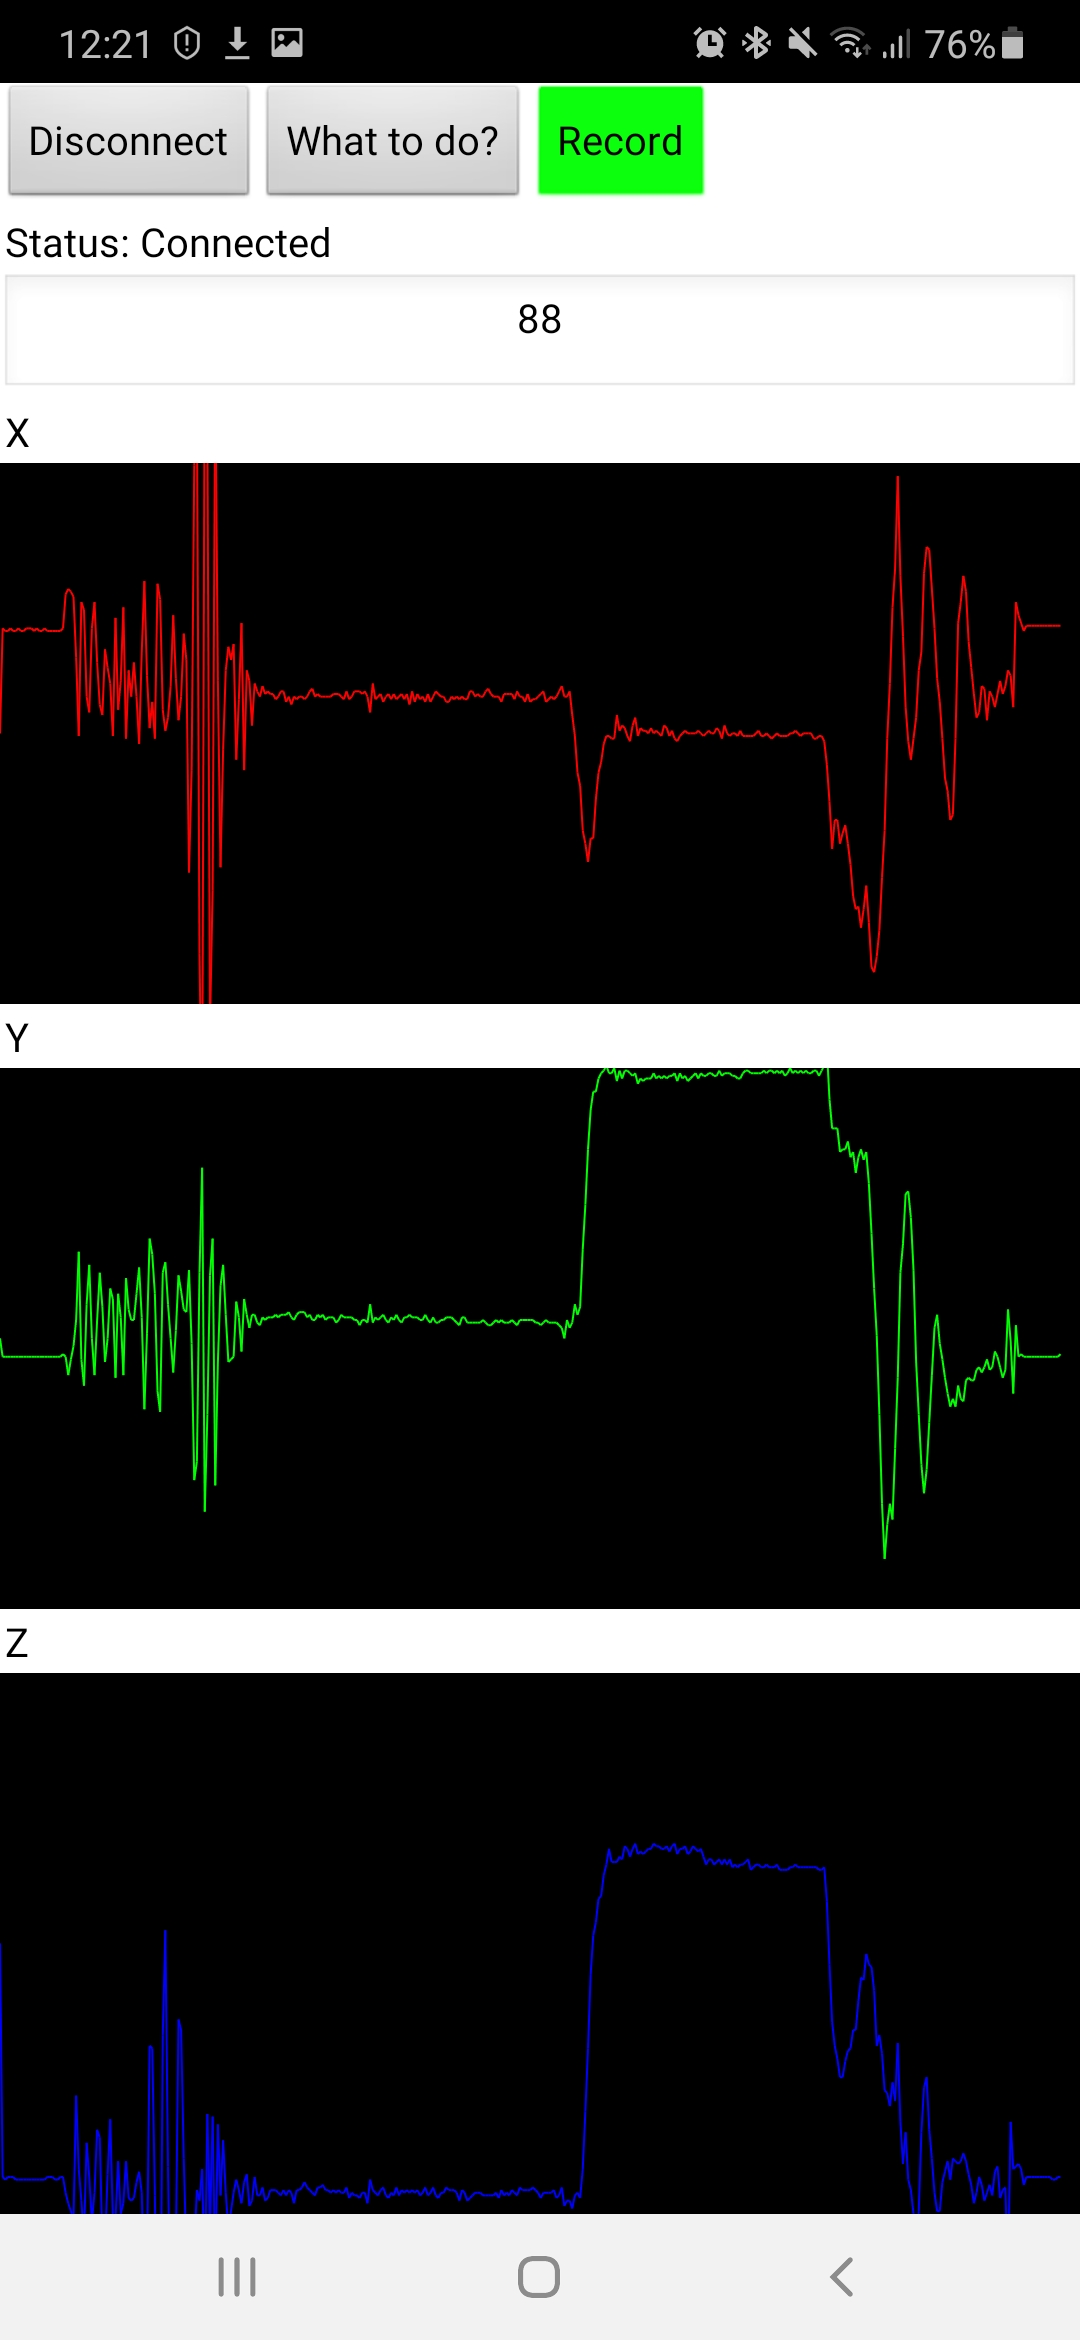
\includegraphics[height=10cm]{Bilder/Graph.jpg}
    \end{minipage}
    \hfill
    \begin{minipage}{0.5\textwidth}
        Die Beschleunigungs-Daten werden in einem Graph dargestellt, hierzu werden sie zuerst in ein
        Array geschrieben. Aus diesem Array erzeugt das Programm in einem vorgegebenen Bereich
        die Datenpunkte, die aufgrund ihrer Masse wie ein Liniendiagramm aussehen.\\
        Neue Daten werden rechts geschrieben, während die alten Daten nach Links aus dem
        Bildschirm verschwinden.\\
        Der Zeitunterschied zwischen Datenpaketen wird in Millisekunden auf dem Bildschirm
        angezeigt.
        Es ist möglich die Daten gleichzeitig aufzuzeichnen.\\
    \end{minipage}
\\

\subsection{Animation}
Hier wird die Distanz aus den Beschleunigungsdaten berechnet und mithilfe eines Punktes
visualisiert. Benutzt werden hierfür die X- und Y-Achse. 
Die Rechnung ist in Kapitel \textit{5.4.1 Gleichmäßige Formel}  beschrieben.

\subsection{Aufgezeichnete Daten}
    \begin{minipage}{0.5\textwidth}
        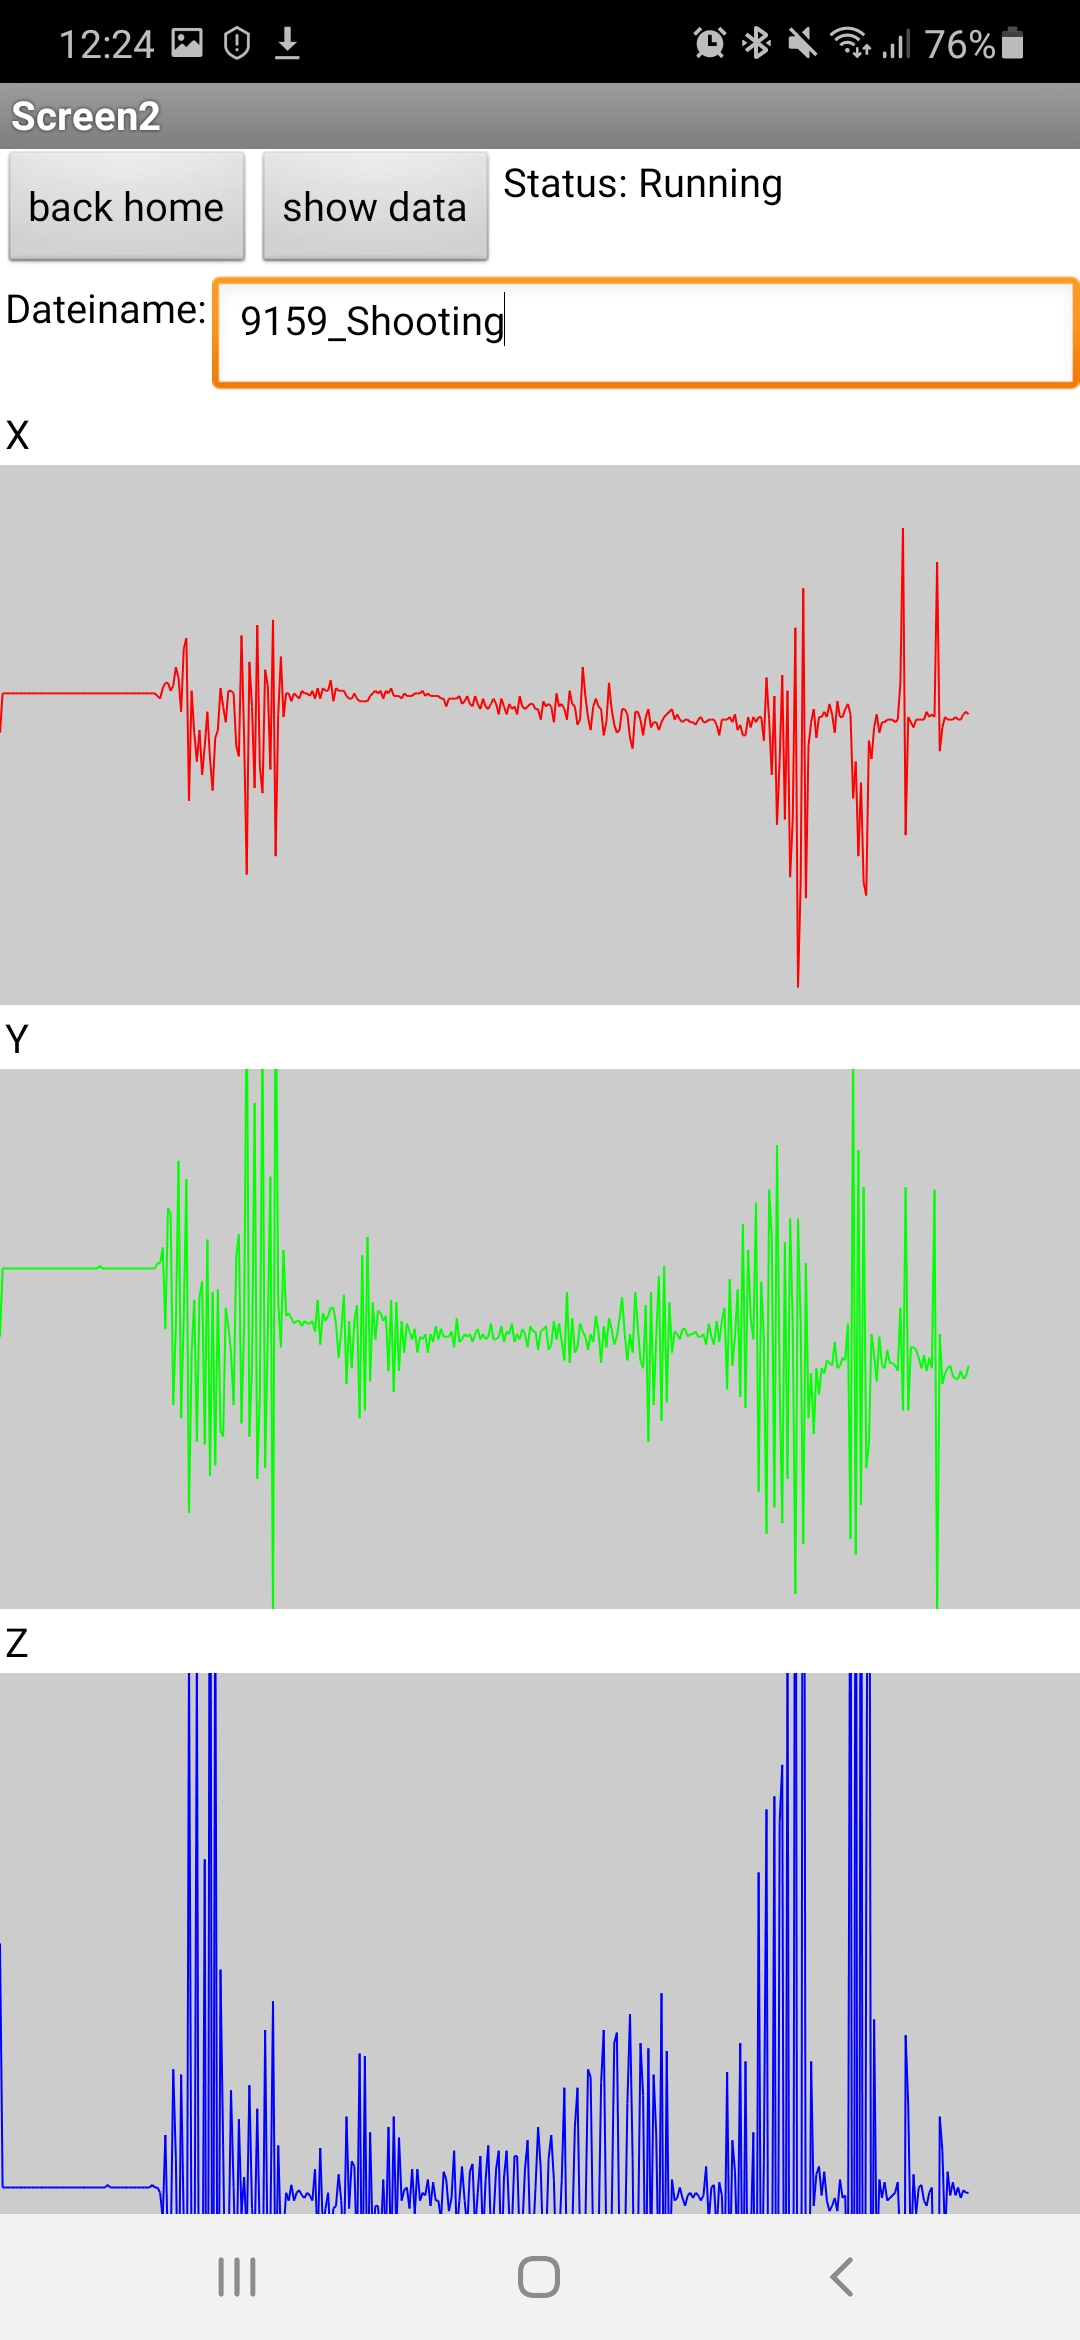
\includegraphics[height=10cm]{Bilder/GraphRec.jpg}
    \end{minipage}
    \hfill
    \begin{minipage}{0.5\textwidth}
        Die von den anderen Funktionen aufgezeichneten Graphen können hier ausgegeben
        werden. Hierzu benötigt der Schütze den Namen der Datei. Die Dateien werden
        seit kurzem unter Android in einem App-eigenen Ordner gespeichert. Diesen muss
        der Schütze momentan auslesen, um den zufälligen Namen der neuen Datei zu kennen.\\
        Die Daten werden als Graph dargestellt. Die Beschleunigungsdaten werden außerdem
        in Rohform über dem Graphen ausgegeben.\\
    \end{minipage}
